\documentclass[tikz,border=10pt]{standalone}
\usetikzlibrary{angles,quotes,intersections,calc}

\begin{document}
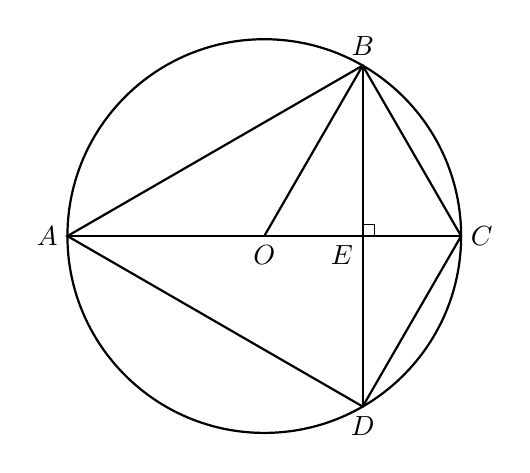
\begin{tikzpicture}
    % 1. 定义基本参数
    \def\R{2.5} % 半径
    \coordinate (O) at (0,0);
    \coordinate (A) at (-\R,0);
    \coordinate (C) at (\R,0);
    
    % 2. 绘制圆
    \draw[thick] (O) circle (\R);
    
    % 3. 定义点 B 和 D (设定角度以符合图片形态)
    \coordinate (B) at (60:\R);
    \coordinate (D) at (-60:\R);
    
    % 4. 定义垂足 E
    \coordinate (E) at ($(A)!(B)!(C)$); % B 在 AC 上的投影
    
    % 5. 绘制所有线条
    \draw[thick] (A) -- (C);
    \draw[thick] (A) -- (B) -- (C) -- (D) -- cycle; % 外轮廓
    \draw[thick] (B) -- (D); % 垂直弦
    \draw[thick] (O) -- (B); % 半径 OB
    
    % 6. 标记直角符号 (使用 right angle 标记)
    \draw (E) rectangle ++(0.15,0.15); 
    
    % 7. 标注点名
    \node[left] at (A) {$A$};
    \node[right] at (C) {$C$};
    \node[above] at (B) {$B$};
    \node[below] at (D) {$D$};
    \node[below] at (O) {$O$};
    \node[below left] at (E) {$E$};
    
\end{tikzpicture}
\end{document}